
\title{MDO via MDF and IDF}

\author{
       Doug Shi-Dong 260466662 \\
       MECH-579 Multidisciplinary Design Optimization\\
        Department of Mechanical Engineering,  McGill University
}
\date{December 16, 2013}

\documentclass[letterpaper,12pt]{article}

\usepackage[%
    left=1in,%
    right=1in,%
    top=0.5in,%
    bottom=1.0in,%
    paperheight=11in,%
    paperwidth=8.5in%
]{geometry}%
\usepackage{listings}
\usepackage{graphicx}
\usepackage{float}
\usepackage[english]{babel}
\usepackage{amsmath}
\usepackage{float}
\usepackage[font=footnotesize,skip=-6pt,justification=centering]{caption}
\captionsetup[table]{skip=2pt}
\usepackage{subcaption}
\usepackage{wrapfig}
\usepackage{amssymb}
\usepackage{multicol}
\usepackage{array}
\usepackage{verbatim}
\usepackage{pgfplotstable, booktabs}
\usepackage{maplestd2e}
\usepackage{CJK}
\usepackage[framed]{mcode}

\addtolength{\parskip}{-4pt}
\setlength{\parindent}{0cm}

\begin{document}
\maketitle

\section{Introduction}
Through a multidisciplinary design feasibility (MDF) and an individual design feasibility (IDF) framework, find the minimum of $f(x,y)$ dictated by $R_1$ and $R_2$.\\

\begin{tabular}{>{\hfill}p{4cm}p{11cm}}
  minimize & $f(x,y)=-20e^{-[(x_1-1)^2+0.25(x_2-1)^2]}+y_1+cos(y_2)$\\
  with respect to & $ x_1,x_2$  $  \epsilon$    $ \mathbb{R}^n$ \\
 where & $R_1(x,y_1(x,y_2)):y_1=-3e^{-[(x_1+1)^2+0.25(x_2+1)^2]}+sin(y_2)$\\
 &$R_1(x,y_2(x,y_1)):y_2=-3e^{-[5(x_1-3)^2+0.25(x_2-3)^2]}+e^{-y_1}$\\
  \multicolumn{2}{c}{} 
\end{tabular}


In the MDF framework, the governing equations are solved by iterating at every optimization iteration. In contrast, the IDF framework solves for target variables to satisfy the governing equation. Having those target values adds a new design variable for every governing equation. The problem statement can then be reformulated by the following.\\

\begin{tabular}{>{\hfill}p{4cm}p{11cm}}
  minimize & $f(x,y^t,y)=-20e^{-[(x_1-1)^2+0.25(x_2-1)^2]}+y_1+cos(y_2)$\\
  with respect to & $ x_1,x_2,y_1^t,y_2^t$  $  \epsilon$    $ \mathbb{R}^n$ \\
 where & $R_1(x,y_1(x,y_2^t)):y_1=-3e^{-[(x_1+1)^2+0.25(x_2+1)^2]}+sin(y_2^t)$\\
 &$R_1(x,y_2(x,y_1^t)):y_2=-3e^{-[5(x_1-3)^2+0.25(x_2-3)^2]}+e^{-y_1^t}$\\
  \multicolumn{2}{c}{} 
\end{tabular}

Since the governing equations are uncoupled, they now behave exactly like equality constraints.\\

The report contains the analysis of the derivatives of the objective function and the use of Quasi-Newton to find the optimum solution.\\

\section{Derivatives}

The derivatives for the IDF are taken at point $(-0.1,-1,1,1)$ for $(x_1,x_2,y_1^t,y_2^t)$. The cost function being a function of 4 design variables, the calculation of the gradient is different. It will now return a vector with 4 elements instead of 2. For the direct and adjoint approach, the partial derivatives differ from the MDF when it comes to the $\displaystyle\frac{\delta f}{ \delta y}$ and the added $\displaystyle\frac{\delta f}{ \delta y^t}$. Figure~\ref{derivatives} and Table~\ref{deri} show the comparison of first and second order finite differences (FD1 and FD2), complex-step(CS) and direct method(DM). The adjoint method(AM) outputs the same results as the DM.

\begin{center}
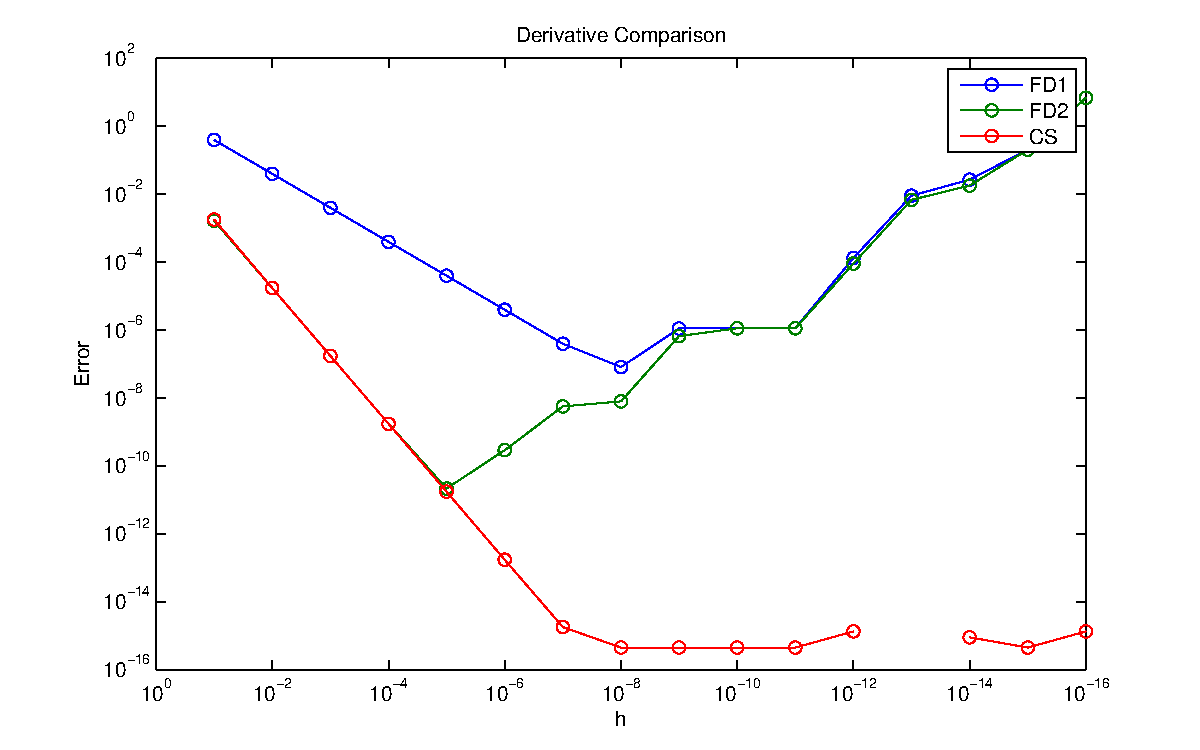
\includegraphics[scale=0.6]{derivatives}
\captionof{figure}{Derivative Comparison}
\label{derivatives}
\end{center}

\begin{table}[h] % Add the following just after the closing bracket on this line to specify a position for the table on the page: [h], [t], [b] or [p] - these mean: here, top, bottom and on a separate page, respectively
\centering % Centers the table on the page, comment out to left-justify
\begin{tabular}{p{1cm} c c c c} % The final bracket specifies the number of columns in the table along with left and right borders which are specified using vertical bars (|); each column can be left, right or center-justified using l, r or c. To specify a precise width, use p{width}, e.g. p{5cm}
\toprule % Top horizontal line
& \multicolumn{4}{c}{$\delta f / \delta x_1$} \\ % Amalgamating several columns into one cell is done using the \multicolumn command as seen on this line
\cmidrule{1-5} % Horizontal line spanning less than the full width of the table - you can add (r) or (l) just before the opening curly bracket to shorten the rule on the left or right side
$\epsilon$ & FD1 & FD2 & CS & DM\\ % Column names row
\midrule % In-table horizontal line
$10^{-1}$ & {\bf-2}.81756819267529 & {\bf-2}.42624843438905 & {\bf-2}.42281111390319 & -2.42459497707862\\
$10^{-2}$ & {\bf-2.4}6403851692807 & {\bf-2.424}61215461720 & {\bf-2.4245}7778649948 & -2.42459497707862\\
$10^{-3}$ & {\bf-2.42}853808035770 & {\bf-2.42459}514891835 & {\bf-2.424594}80523738 & -2.42459497707862\\
$10^{-4}$ & {\bf-2.424}98927222723 & {\bf-2.42459497}879821 & {\bf-2.42459497}536021 & -2.42459497707862\\
$10^{-5}$ & {\bf-2.424}63440645047 & {\bf-2.4245949770}5738 & {\bf-2.4245949770}6144 & -2.42459497707862\\
$10^{-6}$ & {\bf-2.42459}891941493 & {\bf-2.42459497}679093 & {\bf-2.424594977078}45 & -2.42459497707862\\
$10^{-7}$ & {\bf-2.42459}536892170 & {\bf-2.42459497}146186 & {\bf-2.42459497707862} & -2.42459497707862\\
$10^{-8}$ & {\bf-2.42459}505805925 & {\bf-2.4245949}6924141 & {\bf-2.42459497707862} & -2.42459497707862\\
$10^{-9}$ & {\bf-2.42459}607946444 & {\bf-2.42459}563537523 & {\bf-2.42459497707862} & -2.42459497707862\\
$10^{-10}$ & {\bf-2.42459}385901839 &{\bf -2.42459}385901839 &{\bf -2.42459497707862} & -2.42459497707862\\
$10^{-11}$ & {\bf-2.42459}385901839 &{\bf -2.42459}385901839 &{\bf -2.42459497707862} & -2.42459497707862\\
$10^{-12}$ & {\bf-2.424}72708578134 &{\bf -2.4245}0504117642 &{\bf -2.42459497707862} & -2.42459497707862\\
$10^{-13}$ & {\bf-2.4}3360886997834 &{\bf -2.4}3138842392909 &{\bf -2.42459497707862} & -2.42459497707862\\
$10^{-14}$ & {\bf-2}.39808173319034 &{\bf -2.4}4249065417534 &{\bf -2.42459497707862} & -2.42459497707862\\
$10^{-15}$ & {\bf-2}.22044604925031 &{\bf -2}.22044604925031 &{\bf -2.42459497707862} & -2.42459497707862\\
$10^{-16}$ & 4.44089209850063 & 4.44089209850063 & {\bf-2.42459497707862} & -2.42459497707862\\
\bottomrule % Bottom horizontal line
\end{tabular}
\caption{Derivatives Digit Comparison} % Table caption, can be commented out if no caption is required
\label{deri} % A label for referencing this table elsewhere, references are used in text as \ref{label}
\end{table}

From Figure~\ref{derivatives}, we can see that the derivatives are behaving the same way as they did for the MDF. There is no reason the accuracy should be any different. On the other hand, the value of $\delta f / \delta x_1$ is different for the initial point $(-0.1,-1)$, -2.42459497707862 as opposed to 0.0719572647106183, since we are using an initial guess for $y_i$. \\

As it was previously seen in Project 5, for FD1, FD2 and CS, the overall error initially decreases with the perturbation. For the FD methods, the round-off starts to grow and increases the total error as the perturbation decreases further. The CS does not suffer from the round-off error since it is not performing any subtraction of two similar numbers.

\section{Stopping Criterion for IDF}
In order to compare the two methods, we must make sure that they are using equivalent parameters. The convergence for both framework is determined when $\|\nabla f\| <$ 10\text{\sc{e}-}12. For the IDF, the governing equations is converged when reaching 10\text{\sc{e}-}12. Note that even though the IDF is using a constrained optimization, it is not using $\|\nabla \mathcal{L}\| $ to determine convergence. Let's take a look at why we are not using $\|\nabla \mathcal{L}\| $ instead of $\|\nabla f\| $ for the IDF framework.\\

\begin{center}
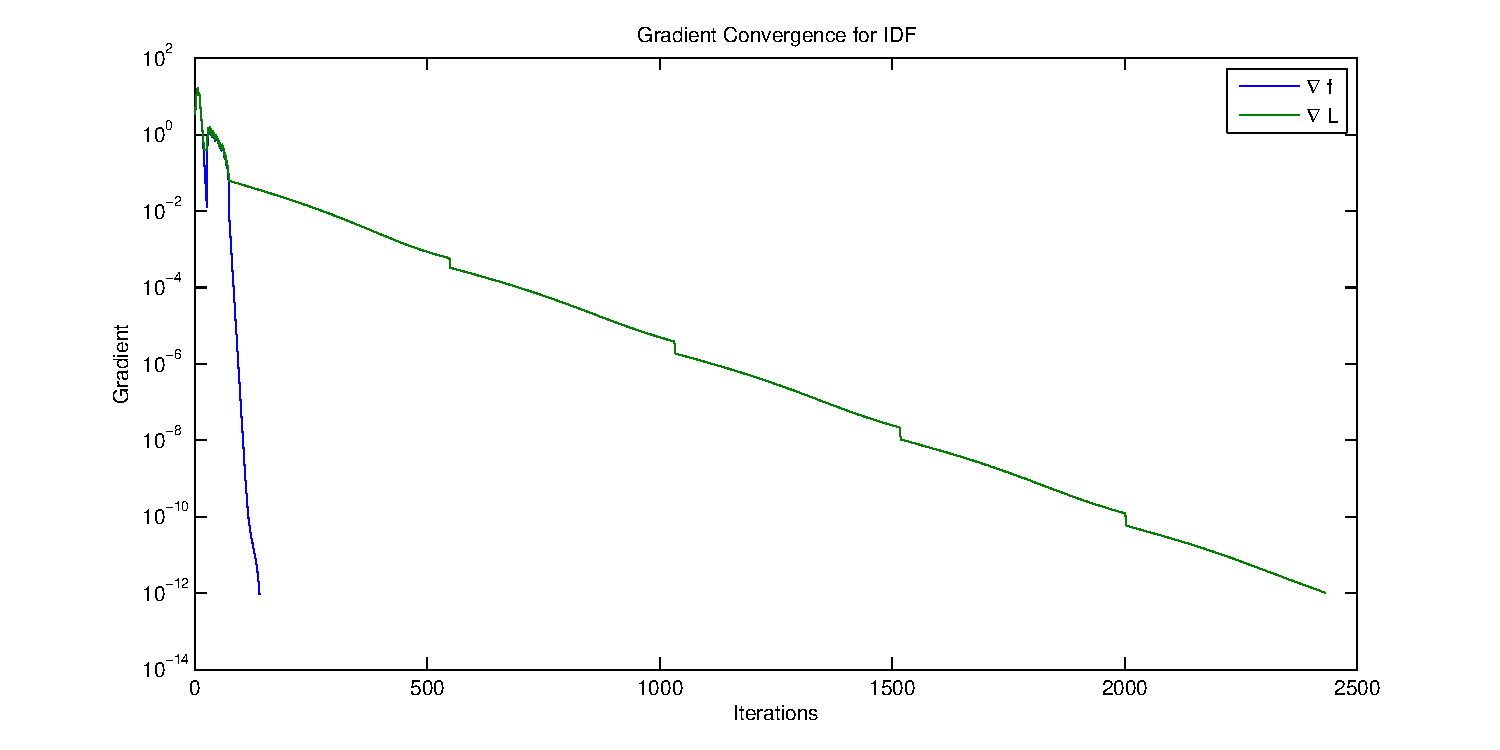
\includegraphics[scale=0.6]{GradCompa}
\captionof{figure}{Stopping Criterion Comparison for IDF}
\label{stopcomp}
\end{center}

The converged values of $x$: \\
$\|\nabla f\| $: $(\textbf{0.997959974383}226, \textbf{0.997959974}646095)$ \\
$\|\nabla \mathcal{L}\| $: $(\textbf{0.997959974383}466,\textbf{0.997959974}866085)$\\

If $\|\nabla \mathcal{L}\|$ is used as the stopping criterion, the change in the values of $x$ stop aftecting the cost function after 140 iterations. However, the target values have not converged to this order. This is because the cost function and governing equations are much more dependent on $x$ than they are on $y$ or $y^t$. Therefore, the gradient will drive the optimization much faster for $x$. Since the step size is the same for every variable, it would require many more iterations in order to converge the Lagrangian. The $\|\nabla \mathcal{L}\|$ is therefore only useful to get a more accurate answer for $y$, not $x$.\\

\section{MDF vs IDF}

Now that we have decided that the gradient of the cost function as a stopping criterion is the better choice for the IDF, we will compare the gradient convergence between the MDF and the IDF. They are both using the starting point $(-0.1,-1)$ for $x$. The IDF uses an initial guess for $y^t$ as $(1,1)$.\\
\newpage
\subsection{Solution}
The first thing we notice is that they have not converged to the same values of $x$:\\
IDF: $(\textbf{0.99}7959974383226, \textbf{0.99}7959974646095)$ \\
MDF: $(\textbf{0.99}8186267926072, \textbf{0.99}8186267761824)$\\

The difference in solution comes from the way the governing equations are calculated. The MDF makes sure that the governing equations are satisfied before moving forward, while the IDF does not. When the optimization is done, the MDF fully respects the governing equations. The IDF has:\\
$y^t=(0.533646333703171,0.576326025500497)$\\
$y$ calculated from target values$=(0.524526128965060,0.586462625580677)$\\
$y$ calculated using $x$ and iterating$=(0.533210261392184,0.586718421462769)$\\

The IDF is less accurate than the MDF since it does not fully respect governing equations. We will see that it leads to some advantages in terms of convergence.

\subsection{Convergence}

\begin{center}
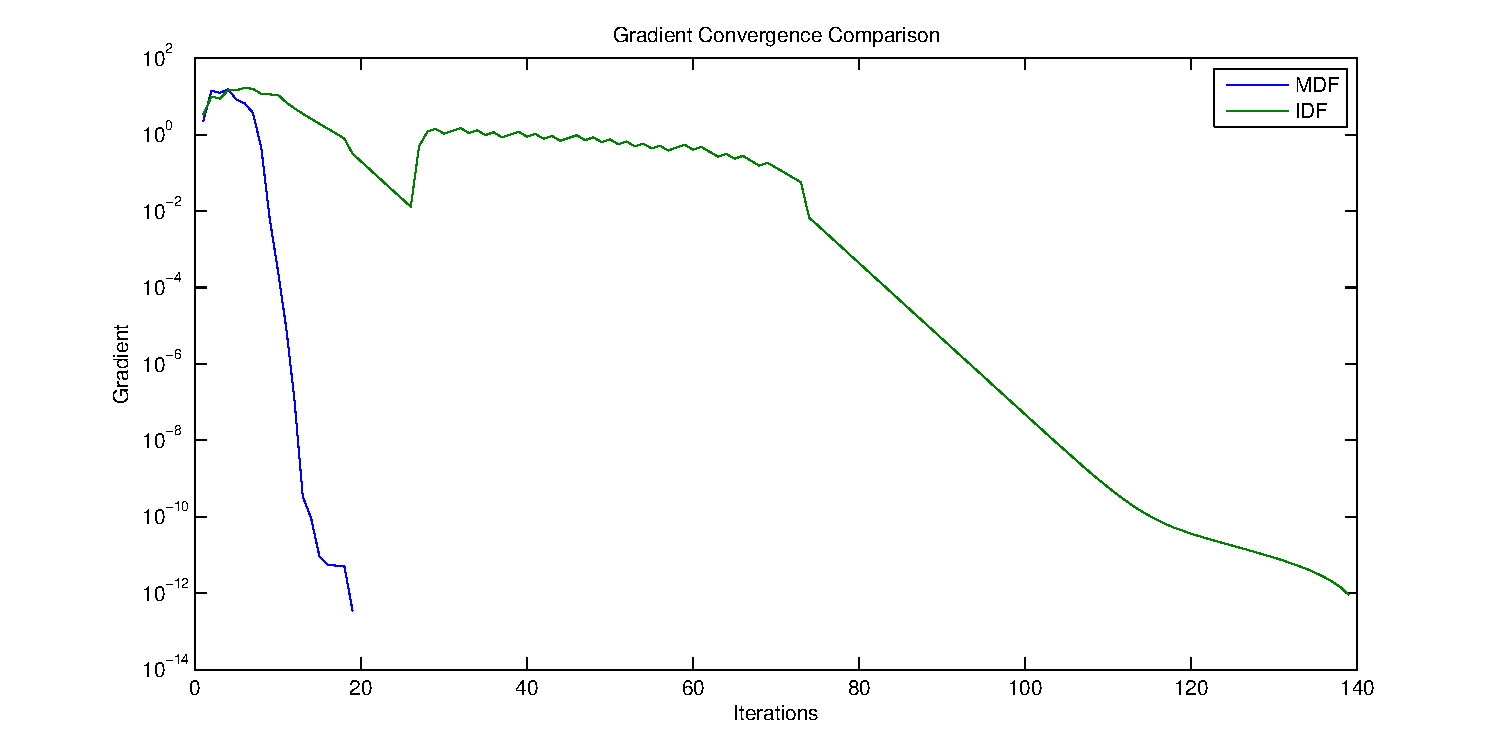
\includegraphics[scale=0.6]{GradConvComp}
\captionof{figure}{Gradient Convergence Comparison}
\label{GradConvComp}
\end{center}

When comparing the gradient convergence, it can be seen that the IDF requires more design cycles. However, it is not the optimization step itself that is costly, but the evaluation of the governing equation. If we take in account the number of times the governing equations have to be solved, the IDF is much less costly. The IDF is required to solve the governing equations 140 times while the MDF requires 1470 iterations.\\

It was assumed that the backtracking algorithm is not required to find the step-size. Therefore, solving the governing equations is only done once at each design cycle for the IDF framework in order to evaluate the cost function. The MDF framework uses a fixed-point iteration at every optimization cycle to find the corresponding $y_i$. The MDF solves the governing equations around 75 times at each design cycle. Despite its quick convergence iteration-wise, the MDF is more costly than the IDF.\\

\subsection{Optimization Path}

\begin{center}
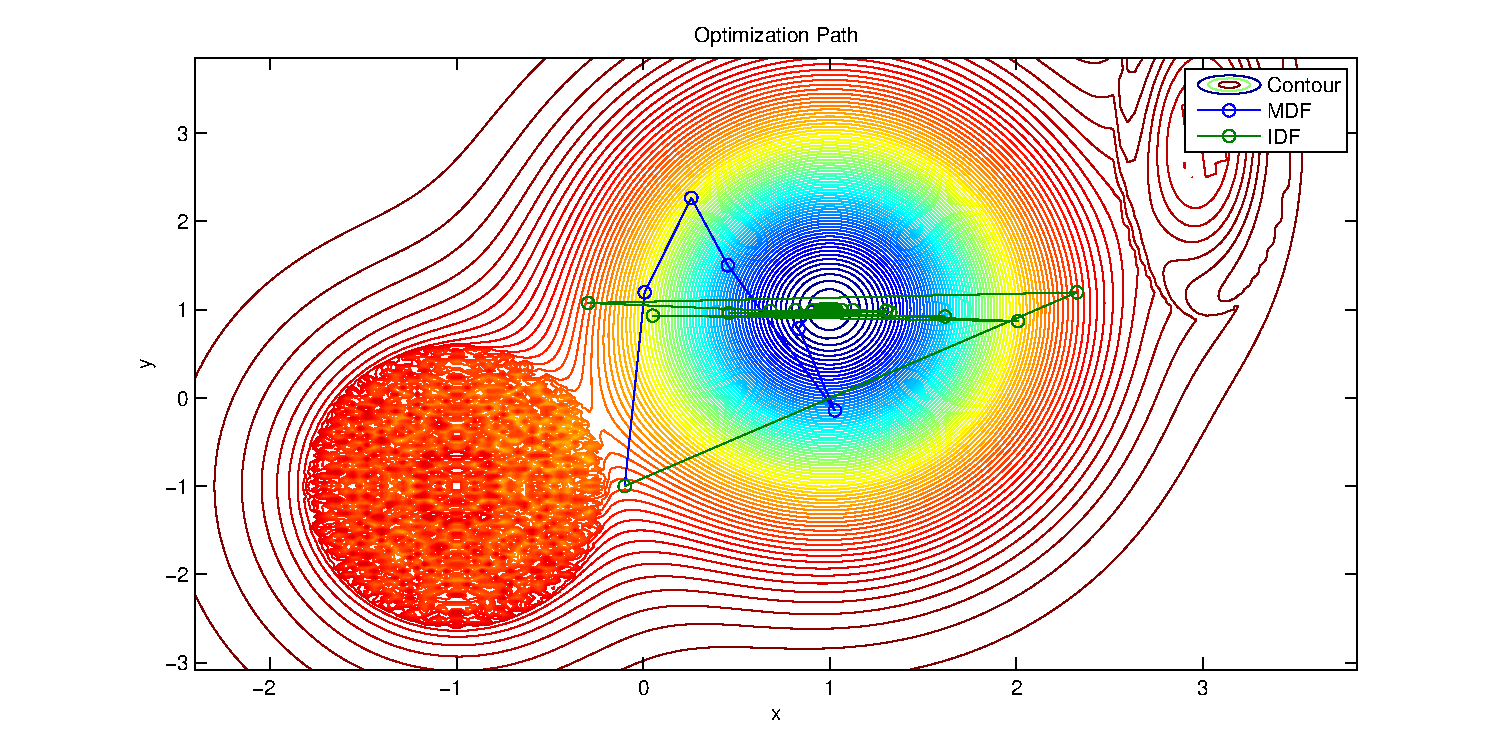
\includegraphics[scale=0.6]{PathComp}
\captionof{figure}{Optimization Path Comparison}
\label{PathComp}
\end{center}

The first thing we notice is that the two paths do not have the same initial direction. That is because of the different $y$'s generated by the $y^t$'s. The MDF path is much more straightforward while the IDF path oscillates back and forth towards the solution. Since the IDF does not have an exact value for $y$, it is constantly adjusting itself as it gets a better idea of what the governing equation values should be.\\

An interesting feature of the IDF is its capability to get out of noisy regions where the governing equations are strongly coupled. Since the governing equations do not have to be satisfied in the early design cycles, it is possible to get out of noisy regions. The MDF was unable to converge to the global minimum and ends up at some other local minimum. The ability to get out of noisy regions is very desirable, especially when solving non-linear systems.
\begin{center}
\begin{multicols}{2}
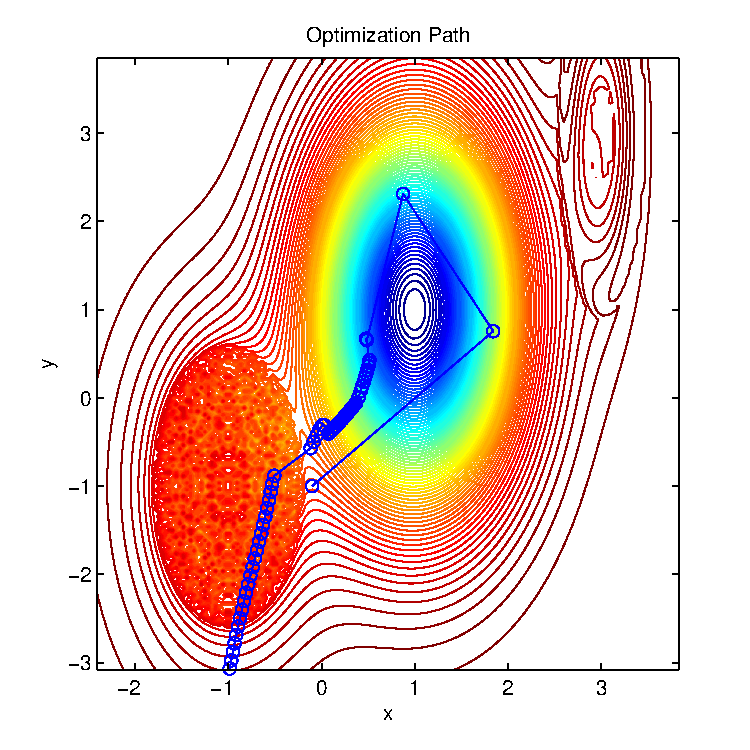
\includegraphics[scale=0.6]{noisyPath}
\captionof{figure}{Optimization Path, Noisy Region}
\label{noisyPath}
\columnbreak
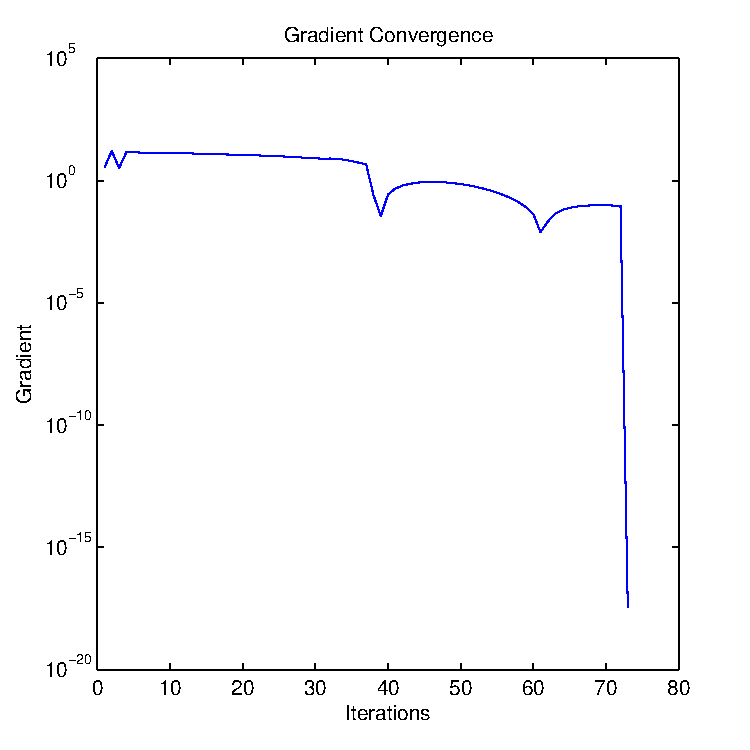
\includegraphics[scale=0.6]{noisyGrad}
\captionof{figure}{Gradient Convergence, Noisy Region}
\label{noisyGrad}
\end{multicols}
\end{center}

\section{Conclusion}

The FD methods decrease in error with the step, but starts increasing when the step becomes small enough for the round-off error to dominate. The CS does not have any round-off error. Those derivatives also confirm the exactitude of the DM and AM.\\

The MDF framework is very expensive because of the necessity to iterate between $y$'s. The IDF requires more design cycle, but it is overall cheaper to compute since it is not iterating between the governing equations. The cheaper cost comes with a price that the solution is less accurate. However, the lower accuracy gives the IDF the ability to get out of noisy regions.\\


\begin{comment}
\newpage
\section{Derivations}
The following derivations have been done on Maple:
%% Created by Maple 16.00, Windows 7
%% Source Worksheet: Untitled (1)
%% Generated: Wed Nov 27 19:23:08 EST 2013
%% Created by Maple 16.00, Windows 7
%% Source Worksheet: Derivations.mw
%% Generated: Wed Nov 27 19:26:04 EST 2013

\def\emptyline{\vspace{12pt}}

\begin{CJK}{}{}
\pagestyle{empty}
\DefineParaStyle{Maple Heading 1}
\DefineParaStyle{Maple Text Output}
\DefineParaStyle{Maple Dash Item}
\DefineParaStyle{Maple Bullet Item}
\DefineParaStyle{Maple Normal}
\DefineParaStyle{Maple Heading 4}
\DefineParaStyle{Maple Heading 3}
\DefineParaStyle{Maple Heading 2}
\DefineParaStyle{Maple Warning}
\DefineParaStyle{Maple Title}
\DefineParaStyle{Maple Error}
\DefineCharStyle{Maple Hyperlink}
\DefineCharStyle{Maple 2D Math}
\DefineCharStyle{Maple Maple Input}
\DefineCharStyle{Maple 2D Output}
\DefineCharStyle{Maple 2D Input}
Definition of objective function f and governing equations R1 and R2

\begin{Maple Normal}{
\begin{Maple Normal}{
}\end{Maple Normal}
}\end{Maple Normal}
\mapleinline{inert}{2d}{f := -20*exp(-(x[1]-1)^2-.25*(x[2]-1)^2)+y[1]+cos(y[2])}{\[\displaystyle f\, := \,-20\,{{\rm e}^{- \left( x_{{1}}-1 \right) ^{2}- 0.25\, \left( x_{{2}}-1 \right) ^{2}}}+y_{{1}}+\cos \left( y_{{2}} \right) \]}
\begin{maplegroup}
\mapleresult
\begin{maplelatex}
\mapleinline{inert}{2d}{-20*exp(-(x[1]-1)^2-.25*(x[2]-1)^2)+y[1]+cos(y[2])}{\[\displaystyle -20\,{{\rm e}^{- \left( x_{{1}}-1 \right) ^{2}- 0.25\, \left( x_{{2}}-1 \right) ^{2}}}+y_{{1}}+\cos \left( y_{{2}} \right) \]}
\end{maplelatex}
\end{maplegroup}
\mapleinline{inert}{2d}{R[1] := -3*exp(-(x[1]+1)^2-.25*(x[2]+1)^2)+sin(y[2])-y[1]}{\[\displaystyle R_{{1}}\, := \,-3\,{{\rm e}^{- \left( x_{{1}}+1 \right) ^{2}- 0.25\, \left( x_{{2}}+1 \right) ^{2}}}+\sin \left( y_{{2}} \right) -y_{{1}}\]}
\begin{maplegroup}
\mapleresult
\begin{maplelatex}
\mapleinline{inert}{2d}{-3*exp(-(x[1]+1)^2-.25*(x[2]+1)^2)+sin(y[2])-y[1]}{\[\displaystyle -3\,{{\rm e}^{- \left( x_{{1}}+1 \right) ^{2}- 0.25\, \left( x_{{2}}+1 \right) ^{2}}}+\sin \left( y_{{2}} \right) -y_{{1}}\]}
\end{maplelatex}
\end{maplegroup}
\mapleinline{inert}{2d}{R[2] := -3*exp(-5*(x[1]-3)^2-.25*(x[2]-3)^2)+exp(-y[1])-y[2]}{\[\displaystyle R_{{2}}\, := \,-3\,{{\rm e}^{-5\, \left( x_{{1}}-3 \right) ^{2}- 0.25\, \left( x_{{2}}-3 \right) ^{2}}}+{{\rm e}^{-y_{{1}}}}-y_{{2}}\]}
\begin{maplegroup}
\mapleresult
\begin{maplelatex}
\mapleinline{inert}{2d}{-3*exp(-5*(x[1]-3)^2-.25*(x[2]-3)^2)+exp(-y[1])-y[2]}{\[\displaystyle -3\,{{\rm e}^{-5\, \left( x_{{1}}-3 \right) ^{2}- 0.25\, \left( x_{{2}}-3 \right) ^{2}}}+{{\rm e}^{-y_{{1}}}}-y_{{2}}\]}
\end{maplelatex}
\end{maplegroup}
\begin{Maple Normal}{
\begin{Maple Normal}{
Partial derivatives of the f}\end{Maple Normal}

}\end{Maple Normal}

\begin{Maple Normal}{
\begin{Maple Normal}{
}\end{Maple Normal}
}\end{Maple Normal}
\mapleinline{inert}{2d}{pfpx1 := diff(f, x[1])}{\[\displaystyle {\it pfpx1}\, := \,{\frac {d}{dx_{{1}}}}f\]}
\begin{maplegroup}
\mapleresult
\begin{maplelatex}
\mapleinline{inert}{2d}{-(20*(-2*x[1]+2))*exp(-(x[1]-1)^2-.25*(x[2]-1)^2)}{\[\displaystyle -20\, \left( -2\,x_{{1}}+2 \right) {{\rm e}^{- \left( x_{{1}}-1 \right) ^{2}- 0.25\, \left( x_{{2}}-1 \right) ^{2}}}\]}
\end{maplelatex}
\end{maplegroup}
\mapleinline{inert}{2d}{}{\[\displaystyle \]}
\mapleinline{inert}{2d}{pfpx2 := diff(f, x[2])}{\[\displaystyle {\it pfpx2}\, := \,{\frac {d}{dx_{{2}}}}f\]}
\begin{maplegroup}
\mapleresult
\begin{maplelatex}
\mapleinline{inert}{2d}{-(20*(-.50*x[2]+.50))*exp(-(x[1]-1)^2-.25*(x[2]-1)^2)}{\[\displaystyle -20\, \left( - 0.50\,x_{{2}}+ 0.50 \right) {{\rm e}^{- \left( x_{{1}}-1 \right) ^{2}- 0.25\, \left( x_{{2}}-1 \right) ^{2}}}\]}
\end{maplelatex}
\end{maplegroup}
\mapleinline{inert}{2d}{pfpy1 := diff(f, y[1])}{\[\displaystyle {\it pfpy1}\, := \,{\frac {d}{dy_{{1}}}}f\]}
\begin{maplegroup}
\mapleresult
\begin{maplelatex}
\mapleinline{inert}{2d}{1}{\[\displaystyle 1\]}
\end{maplelatex}
\end{maplegroup}
\mapleinline{inert}{2d}{pfpy2 := diff(f, y[2])}{\[\displaystyle {\it pfpy2}\, := \,{\frac {d}{dy_{{2}}}}f\]}
\begin{maplegroup}
\mapleresult
\begin{maplelatex}
\mapleinline{inert}{2d}{-sin(y[2])}{\[\displaystyle -\sin \left( y_{{2}} \right) \]}
\end{maplelatex}
\end{maplegroup}
\begin{Maple Normal}{
\begin{Maple Normal}{
Partial derivatives of governing equations f}\end{Maple Normal}

}\end{Maple Normal}

\begin{Maple Normal}{
\begin{Maple Normal}{
}\end{Maple Normal}
}\end{Maple Normal}
\mapleinline{inert}{2d}{pR1px1 := diff(R[1], x[1])}{\[\displaystyle {\it pR1px1}\, := \,{\frac {d}{dx_{{1}}}}R_{{1}}\]}
\begin{maplegroup}
\mapleresult
\begin{maplelatex}
\mapleinline{inert}{2d}{-(3*(-2*x[1]-2))*exp(-(x[1]+1)^2-.25*(x[2]+1)^2)}{\[\displaystyle -3\, \left( -2\,x_{{1}}-2 \right) {{\rm e}^{- \left( x_{{1}}+1 \right) ^{2}- 0.25\, \left( x_{{2}}+1 \right) ^{2}}}\]}
\end{maplelatex}
\end{maplegroup}
\mapleinline{inert}{2d}{pR1px2 := diff(R[1], x[2])}{\[\displaystyle {\it pR1px2}\, := \,{\frac {d}{dx_{{2}}}}R_{{1}}\]}
\begin{maplegroup}
\mapleresult
\begin{maplelatex}
\mapleinline{inert}{2d}{-(3*(-.50*x[2]-.50))*exp(-(x[1]+1)^2-.25*(x[2]+1)^2)}{\[\displaystyle -3\, \left( - 0.50\,x_{{2}}- 0.50 \right) {{\rm e}^{- \left( x_{{1}}+1 \right) ^{2}- 0.25\, \left( x_{{2}}+1 \right) ^{2}}}\]}
\end{maplelatex}
\end{maplegroup}
\mapleinline{inert}{2d}{pR1py1 := diff(R[1], y[1])}{$\displaystyle {\it pR1py1}\, := \,{\frac {d}{dy_{{1}}}}R_{{1}}$}
\mapleinline{inert}{2d}{}{$\displaystyle $}
\begin{maplegroup}
\mapleresult
\begin{maplelatex}
\mapleinline{inert}{2d}{-1}{\[\displaystyle -1\]}
\end{maplelatex}
\end{maplegroup}
\mapleinline{inert}{2d}{pR1py2 := diff(R[1], y[2])}{\[\displaystyle {\it pR1py2}\, := \,{\frac {d}{dy_{{2}}}}R_{{1}}\]}
\begin{maplegroup}
\mapleresult
\begin{maplelatex}
\mapleinline{inert}{2d}{cos(y[2])}{\[\displaystyle \cos \left( y_{{2}} \right) \]}
\end{maplelatex}
\end{maplegroup}
\mapleinline{inert}{2d}{pR2px1 := diff(R[2], x[1])}{\[\displaystyle {\it pR2px1}\, := \,{\frac {d}{dx_{{1}}}}R_{{2}}\]}
\begin{maplegroup}
\mapleresult
\begin{maplelatex}
\mapleinline{inert}{2d}{-(3*(-10*x[1]+30))*exp(-5*(x[1]-3)^2-.25*(x[2]-3)^2)}{\[\displaystyle -3\, \left( -10\,x_{{1}}+30 \right) {{\rm e}^{-5\, \left( x_{{1}}-3 \right) ^{2}- 0.25\, \left( x_{{2}}-3 \right) ^{2}}}\]}
\end{maplelatex}
\end{maplegroup}
\mapleinline{inert}{2d}{pR2px2 := diff(R[2], x[2])}{\[\displaystyle {\it pR2px2}\, := \,{\frac {d}{dx_{{2}}}}R_{{2}}\]}
\begin{maplegroup}
\mapleresult
\begin{maplelatex}
\mapleinline{inert}{2d}{-(3*(-.50*x[2]+1.50))*exp(-5*(x[1]-3)^2-.25*(x[2]-3)^2)}{\[\displaystyle -3\, \left( - 0.50\,x_{{2}}+ 1.50 \right) {{\rm e}^{-5\, \left( x_{{1}}-3 \right) ^{2}- 0.25\, \left( x_{{2}}-3 \right) ^{2}}}\]}
\end{maplelatex}
\end{maplegroup}
\mapleinline{inert}{2d}{pR2py1 := diff(R[2], y[1])}{\[\displaystyle {\it pR2py1}\, := \,{\frac {d}{dy_{{1}}}}R_{{2}}\]}
\begin{maplegroup}
\mapleresult
\begin{maplelatex}
\mapleinline{inert}{2d}{-exp(-y[1])}{\[\displaystyle -{{\rm e}^{-y_{{1}}}}\]}
\end{maplelatex}
\end{maplegroup}
\mapleinline{inert}{2d}{pR2py2 := diff(R[2], y[2])}{\[\displaystyle {\it pR2py2}\, := \,{\frac {d}{dy_{{2}}}}R_{{2}}\]}
\begin{maplegroup}
\mapleresult
\begin{maplelatex}
\mapleinline{inert}{2d}{-1}{\[\displaystyle -1\]}
\end{maplelatex}
\end{maplegroup}
\begin{Maple Normal}{
\begin{Maple Normal}{
\mapleinline{inert}{2d}{}{$\displaystyle $}
}\end{Maple Normal}
}\end{Maple Normal}
\begin{Maple Normal}{
\begin{Maple Normal}{
\mapleinline{inert}{2d}{}{\[\displaystyle \]}
}\end{Maple Normal}
}\end{Maple Normal}
\end{CJK}


The following statements are in MATLAB to compute the derivatives:\\

{\bf Direct Method:}\\

A=[pR1py1 pR1py2; pR2py1 pR2py2];\\
Ainv=inv(A);\\

dydx(:,1)=-Ainv*[pR1px(1);pR2px(1)];\\
dydx(:,2)=-Ainv*[pR1px(2);pR2px(2)];\\

dfdx(1)=pfpx(1)+pfpy1*dydx(1,1)+pfpy2*dydx(2,1);\\
dfdx(2)=pfpx(2)+pfpy1*dydx(1,2)+pfpy2*dydx(2,2);\\

dfdx=dfdx';\\

{\bf Adjoint Method:}\\

A=[pR1py1 pR2py1;pR1py2 pR2py2];\\
Ainv=inv(A);\\

psi=-Ainv*[pfpy1;pfpy2];\\

dfdx(1)=pfpx(1)+psi(1)*pR1px(1)+psi(2)*pR2px(1);\\
dfdx(2)=pfpx(2)+psi(1)*pR1px(2)+psi(2)*pR2px(2);\\

dfdx=dfdx';\\

\end{comment}

\newpage
\section*{Derivation}
All the derivations have been done in Maple. In the following code, $\delta y^t$ are designed by *px(3) and *px(4)
\lstinputlisting{directD.m}


\end{document}
